
\documentclass[a4paper, oneside]{sapthesis}
% ---- DRAFT SWITCH ----
\newif\ifdraft
\draftfalse      % <-- DURANTE LA STESURA (veloce)
% \draftfalse   % <-- PER LA VERSIONE FINALE (lenta ma completa)
% --------------
\usepackage{microtype}     
\usepackage[utf8]{inputenc}
\usepackage[english]{babel}
\usepackage{csquotes}
\usepackage{imakeidx}
\usepackage{graphicx}
\graphicspath{{immagini/}} 
\DeclareGraphicsExtensions{.png,.pdf,.jpg}
\captionsetup{labelsep=quad}
\usepackage{array}
\usepackage{ragged2e}
\usepackage[table]{xcolor}
\usepackage{hyperref}
\usepackage{blindtext}
\usepackage[style=apa, backend=biber, sortcites=true, sorting=nyt]{biblatex} 

\usepackage{placeins}
\usepackage{caption} 
\usepackage{subcaption}
\usepackage{float}
\renewcommand{\topfraction}{0.9}
\renewcommand{\textfraction}{0.05}
\renewcommand{\floatpagefraction}{0.8}
\addbibresource{bibliografia.bib}
% Se usi english:
\DeclareLanguageMapping{english}{english-apa}
\DeclareFieldFormat[article]{volume}{\apanum{#1}} % Format volume number
% Graphicx + modalità draft immagini

\ifdraft
  \PassOptionsToPackage{draft}{graphicx} % riquadri al posto delle figure (molto veloce)
\fi
\graphicspath{{immagini/}}
\DeclareGraphicsExtensions{.png,.pdf,.jpg}


% Modify 'and' to '&' in the bibliography
\renewcommand*{\finalnamedelim}{%
  \ifnumgreater{\value{liststop}}{2}{\finalandcomma}{}%
  \addspace\&\space}
\usepackage[linguistics]{forest} %per dare i diagrammi: https://texdoc.org/serve/forest/0

\newcommand*{\belowrulesepcolor}[1]{% 
  \noalign{% 
  \kern-\belowrulesep \begingroup \color{#1}% 
  \hrule height\belowrulesep \endgroup }%
}
\newcommand*{\aboverulesepcolor}[1]{% 
  \noalign{%
  \begingroup \color{#1}% 
  \hrule height\aboverulesep \endgroup \kern-\aboverulesep }%
}




\hypersetup{pdftitle={TITOLO TESI}, pdfauthor={Alessandra Amicucci}}
\title{TITOLO TESI}
\author{Alessandra Amicucci}
\IDnumber{1940795}
\course{Master Degree in Economics and policy evaluation}
\courseorganizer{Facoltà di Economia}
\AcademicYear{2024/2025}
\advisor{Dott. Valerio Leone Sciabolazza}
\customadvisorlabel{Supervisor}
%\coadvisor{Dott.ssa Nome Cognome}
%\customcoadvisorlabel{Correlatrice}
%\director{Dott.  Nome Cognome}
%\customdirectorlabel{Specializzando\\Responsabile della ricerca}
\authoremail{email amicucci.1940795@studenti.uniroma1.it}
\copyyear{2025}


%In caso di titoli di section a 2 righe
%\setlength{\headheight}{22.59052pt}
%\addtolength{\topmargin}{-10.59052pt}

\makeindex
\includeonly{Cap_1,Cap_2,Cap_3,Cap_4,Cap_5,appendix}
\newcommand{\Fig}[1]{[{\footnotesize \texttt{Fig.#1}}]}
\newcommand{\citfig}[1]{\ap{\scriptsize\textrm{(\textit{F#1})}}}

\begin{document}
\frontmatter
\maketitle
\dedication{Dedicato a SCRIVI QUI LA DEDICA }

\begin{abstract}
This thesis studies how exposure to international maritime trade shapes subnational conflict in Nigeria. For doing so, we built an exposure to trade index. We interacted changes in container port throughput (CPT) with the Liner Shipping Connectivity Index (LSCI) and the inverse distance to the nearest commercial port. Then, we studies the effect of the trade index to conflict, in particular ADM2 level events from ACLED (2009–2019). Using two-way fixed effects we found that higher exposure to trade is associated with a stabilizing effect on conflicts at the micro level, especially in poorer areas, while effects are near zero or weaker in more developed districts. Accounting for heterogeneity, results reported a stronger effect in the eastern coastal regions and for ports oriented toward vegetable goods and imports, and they attenuate in regions with abundance of water availability, a proxy for agricultural rents, aligning with the result of the baseline model. We continued the analysis estimating a falsification test using non-commercial ports and that supported our main hypothesis, demonstrating an effect of trade in conflict, rather than mere geographic proximity. The findings highlights the central role of pre-existing economic and spatial inequalities in mediating the stabilizing effects of globalization

\end{abstract}
%\tableofcontents
%\listoffigures
%\listoftables

\phantomsection
%\addcontentsline{toc}{chapter}{Acronomi}

\mainmatter
\chapter{Introduzione}
\section{Motivation and Index Construction}

While a vast literature has explored the effects of trade liberalization in developed economies, less is known about its consequences in developing countries, particularly concerning internal stability and conflict. In these contexts, trade represents a major channel through which global economic fluctuations are transmitted to local welfare and political stability \parencite{united2011review}. Existing research has often examined related mechanisms through the lens of commodity price shocks. For instance, \textcite{dube2013commodity} and \textcite{bruckner2010international} analyse how international price variations affect conflict outcomes, finding mixed results depending on the type of resource and the institutional environment. Other contributions have instead focused on the reverse relationship, investigating how conflict disrupts trade flows and economic integration \parencite{martin2008civil}. 
However, evidence on how trade shocks themselves, rather than price or conflict shocks—affect local stability remains limited, especially at the subnational level in low- and middle-income countries. Our analysis addresses this gap by examining how spatial exposure to trade integration shapes conflict dynamics within Nigeria, combining detailed information on port activity, global connectivity, and local socio-economic characteristics.
Our analysis builds on the intuition of \textcite{berman2015external}, who show that positive income shocks, such as those generated by trade, can reduce conflict by improving local economic opportunities. Conversely, trade can also exacerbate tensions when it increases the value of contestable rents or reinforces existing inequalities, as shown by \textcite{amodio2024trade}. These dual mechanisms, often referred to as the \textit{opportunity} or \textit{income} and \textit{rent-seeking} effects, suggest that the impact of trade on conflict is theoretically ambiguous and context-dependent.

Nigeria represents an ideal setting to study these dynamics. It is a coastal country with a diversified set of ports and abundant natural resources, where trade-related income shocks can have significant spatially heterogeneous effects. Its geography—marked by strong North–South disparities and localized ethnic divisions—makes it a relevant case for testing whether trade integration promotes peace or amplifies existing inequalities.

To empirically assess these mechanisms, we construct a spatial trade exposure index inspired by shift–share approaches. The index combines three main components:
\begin{enumerate}
	\item \textbf{Trade shocks}, measured as annual changes in port-level container throughput from IMF PortWatch;
	\item \textbf{Connectivity}, proxied by the Liner Shipping Connectivity Index (LSCI) from UNCTAD, which captures each port’s integration in global maritime networks;
	\item \textbf{Proximity}, expressed as the inverse distance between each ADM2 centroid and the nearest port (including Onne, added to complement the FAO–UNCTAD list).
\end{enumerate}

INDEX
This formulation captures how strongly each subnational unit is exposed to international trade shocks depending on its geographical proximity and the global relevance of its nearest ports. Regions located closer to active and well-connected ports are assumed to experience stronger transmission of trade-related income shocks.

Our contribution is twofold. First, we provide one of the first subnational evaluations of trade shocks and conflict in Africa, combining spatially detailed datasets on trade, conflict, infrastructure, and environmental factors. Second, we show that the effect of trade openness is highly heterogeneous: while it fosters stability in resource-constrained and less developed areas, it may reinforce instability in already prosperous or rent-dependent regions. These findings highlight the importance of considering spatial inequality in designing conflict-sensitive trade and infrastructure policies.

\chapter{Data}
In our empirical analysis, we combined different data sources to derive a panel of subnational geographical units for the period from 2009 to 2019. Data on conflict event are drawn from the "Armed Conflict and Location Event" (ACLED) which cover conflict event from 1999 to 2024. The dataset provides the exact location of events, the type of event, and other characteristics related to the conflict. \cite{raleigh2010introducing}
In constructing the dataset, we focused on consumption-related conflict events rather than rapacity-based events. Both theoretical and empirical considerations guide this choice. Trade openness influences a country's income, usually in a positive way. However, globalisation has not always reduced inequalities in emerging countries, causing unequal distribution. 
As stated by \textcite{dube2013commodity}, an increase in income can reduce conflict, but on the other hand, higher income means there is more to fight over these resources. The existence of two opposing influences, opportunity cost and rapacity, suggests that some shocks may mitigate conflict, whereas other shocks exacerbate it, depending on the relative strength of the two effects.
The study of \textcite{amodio2024trade} shows that exposure to exports increasess simultaneously economic activity and political violence. Meanwhile, \textcite{mcguirk2020economic} have shown that, in the event of positive price shocks, producers' revenues increase but consumers' real incomes decrease, thus enhancing the probability of protests or demonstrations. Consumption-related mechanisms are more directly influenced by exogenous trade shocks, while conflicts over resources follow different dynamics, often linked to the strategies of armed groups. From an empirical point of view, limiting oneself to consumption-related events also mitigates concerns about endogeneity: resource predation can in itself influence local trade flows, risking to reflect both cause and effect simultaneously.

The final variable therefore measures the annual number of consumption-related conflict events for ADM2, filtered to retain only: (i) subcategories of events not related to predation, such as protests (peaceful or violent), demonstrations, arrests, agreements or territorial changes not directly linked to resource predation. (ii) Events reported in narrative notes as disputes over consumer goods or livelihoods (keywords such as land, livestock, pasture, farm, grazing, oil, gold, looting).
Events clearly associated with predatory motives (e.g., looting, armed clashes over resource extraction, kidnappings for ransom) are excluded.

After filtering, we limited the dataset to events occurring in coastal regions, then projected them into a consistent spatial reference system and overlaid them on Nigeria's second-level administrative units (ADM2). For each ADM2-year, the count of non-predatory conflict events is available, which serves as the outcome variable in my regression analysis.
\chapter{Methodoloy}

We expect the economic impact of trade shocks to vary across different ADM2 units, with areas most exposed to international trade experiencing fewer consumption-related conflict events. Following this intuition, the index presented in the chapter Data was constructed, combining two national components that vary over time with a fixed spatial component. This approach is consistent with consolidated practices in the literature that combine aggregate shocks with sub-national heterogeneity \parencite{autor2013china}.\\

The mechanism linking trade exposure and conflict is consistent with the opportunity-cost and grievance framework discussed by \textcite{amodio2021security}. Their evidence suggests that economic integration and access to trade can shape local conflict dynamics by altering individuals’ economic incentives and perceptions of welfare.
In this thesis, the focus is on the opposite mechanism: instead of trade restrictions, we study whether higher trade openness and proximity to maritime ports, which expand local economic opportunities, can mitigate the incidence of violence. The same channels highlighted by \textcite{amodio2021security} are therefore expected to operate in reverse, with improved trade connectivity reducing both grievance and the opportunity to engage in conflict.

\section{Conceptual framework}
To better capture the mechanisms through which trade exposure affects social stability, we construct a specific subset of conflict events reflecting consumption- or income-related tensions rather than resource-seeking or political violence. Starting from the ACLED dataset \parencite{acled2025}, we select events classified as protests or demostrations, the types less likely to have a link with resource predation. In particular, we identify income-related events through a keyword-based text filter, selecting those that mention terms associated with basic-needs or livelihood shocks, such as food, fuel, price, subsidy, market, ration, maize, rice, bread, or tax.
Conflict incidence can be represented as \eqref{conflict} where $Y_{it}$ captures opportunity-income effects (the effect of trade in income, reducing conflict) and $R_{it}$ captures rent-seeking incentives (the opposite effect of trade that incentivises conflict).
\begin{equation}
	Conflict_{it} = f(Y_{it}, R_{it})
	\label{conflict}
\end{equation}
Our index captures exogenous variation in the income effect transmitted through trade shocks, holding the incentives largely constant by excluding rapacity-related events.

\section{Identification Strategy}
Identification relies on within district (ADM2) variation in exposure to national trade shocks over time. Because the trade shock (CPT × LSCI) is common across units while the distance is time-invariant, only the interaction between these components generates differential effects once ADM2 and year fixed effects are included. 
In our case, the CPT was delayed by one year to mitigate possible simultaneity issues, while the LSCI represents the degree of integration of the Nigerian port system into global maritime networks. Spatial heterogeneity is introduced through the minimum distance from ports, which serves as a proxy for accessibility to international markets. Following the intuition of \parencite{berman2015external}, regions located closer to ports are more directly integrated into international trade networks and therefore more strongly affected by external shocks. In our context, this motivates the use of minimum distance from ports as a measure of local exposure, assuming that trade shocks are transmitted more intensely to areas with better access to maritime infrastructure.
In this sense, the empirical design is consistent with the validity conditions discussed by \parencite{goldsmith2020bartik}\\
The empirical model also includes both spatial (ADM2) and temporal (year) fixed effects. In this way, given the same national shock, only differences in proximity to ports generate variation between units, allowing the heterogeneous effect of trade shocks on conflict to be isolated. 
To account for spatial heterogeneity the distances from ports where normalised. Since the relationship between trade exposure and conflict is expected to decrease with distance, the raw distances (measured in kilometers) were first inverted to capture proximity rather than remoteness. To ensure comparability across regions, the proximity measure was then rescaled between 0 and 1, so that values closer to 1 represent areas with higher accessibility to maritime trade. This transformation preserves relative spatial differences while avoiding scale distortions that could bias the exposure index.

\section{Empirical Strategy}
All models are estimated using OLS with two-way fixed effects (ADM2 and year). Standard errors are clustered at the ADM2 level to account for serial correlation within units over time. 
The empirical strategy consists of three steps.
\textit{First}, we estimate the basic model in two specifications: an aggregate version, in which the exposure index is considered in its overall form (Equation\eqref{eq1}), and a “split” version, which distinguishes administrative units based on the intensity of economic development measured by night-time lights (Equation \eqref{eq2}). This allows us to analyse both the average effect of the trade shock and the differences between more and less developed areas.\\
\begin{equation}
	Conflict_{it} = \beta Index_{it} + \gamma log(Nightlights_{it}) + \mu_i + \lambda_t + \varepsilon_{it}
	\label{eq1}
\end{equation}
\begin{equation}
	Conflict_{it} = \beta_1 Index_{it}^{HigNL}+ \beta_2 Index_{it}^{LowNL}+ \gamma log(Nightlights_{it}) + \mu_i + \lambda_t + \varepsilon_{it}
	\label{eq2}
\end{equation}
\textit{Second}, we perform a falsification test to verify that the results do not simply reflect a spurious correlation between conflict and geographical proximity to port infrastructure. To this end, we reconstruct the index to include all ports in Nigeria, not just commercial ones. The idea is that if the effect were linked exclusively to physical proximity to a port, it should also emerge with this broader measure. Conversely, if the association is really driven by trade shocks, the results should only appear when considering ports that are actually relevant to international trade.\\
\textit{Third}, beyond the baseline model, we explore whether the trade–conflict relationship varies across key structural dimensions. Following the idea that the effects of economic integration depend on pre-existing territorial and social characteristics (\parencite{berman2015external}), we analyse the heterogeneity of the effects across region, sector and environment. 
In particular, we distinguish between (i) eastern and western regions, (ii) the predominant type of industry traded, (iii) the predominant trade flow and (iv) water availability. These specifications allow us to investigate the differentiated transmission of trade shocks depending on the structural conditions of the territories. Equation \ref{eq:heterogeneity} extends the baseline model to account for heterogeneity across structural or environmental dimensions.
The interaction term captures whether the effect of trade exposure differs depending on regional location or sectoral specialization. A negative and statistically significant coefficient on $\beta_2$  would indicate that the pacifying effect of trade is stronger in the corresponding subgroup.
\begin{equation}
	Conflict_{it} = \beta_1 Index_{it} + \beta_2 (Index_{it} \times H_i) + \gamma \log(Nightlights_{it}) + \mu_i + \lambda_t + \varepsilon_{it}
	\label{eq:heterogeneity}
\end{equation}

Equation \ref{eq:heterogeneity} account for water availability heterogeneity. $HighWater$ and $LowWater$ are dummies equal to one for ADM2 units above or below the median of the FAO–GAEZ water-availability distribution.
In this analysis the coefficients $\beta2$ and $\beta3$ capture how the trade–conflict relationship differs across regions with different quantity of water resources
\begin{equation}
	\begin{aligned}
		Conflict_{it} &= \beta_1 Index_{it} 
		+ \beta_2 (Index_{it} \times HighWater_i)
		+ \beta_3 (Index_{it} \times LowWater_i) \\
		&\quad + \gamma \log(Nightlights_{it})
		+ \mu_i + \lambda_t + \varepsilon_{it}
	\end{aligned}
	\label{eq:water_hetero}
\end{equation}




\chapter{Results}
In what follows, we present three sets of results. First we studied the baseline model estimating the effect of the trade exposure index in conflict taking into account the economic heterogeneity. Second we show the model taking into account the geographical, sectorial and tribal heterogeneity. Third, we investigate the effect of the index across region with different water availability. \\

\section{Baseline model}
Table\ref{tab:ports_main} reports the estimates of the main coefficient from Equation \eqref{eq1} and \eqref{eq2}.
\begin{table}[htbp]
	\centering
	\caption{Correlation between port shocks and conflict: commercial vs all ports}
	\label{tab:ports_main}
	\begingroup
	\def\sym#1{\ifmmode^{#1}\else\(^{#1}\)\fi}
	\begin{adjustbox}{max width=\textwidth}
		\begin{tabular}{lcccc}
			\toprule
			& (1) Commercial ports & (2) Commercial ports & (3) All ports & (4) All ports \\
			\midrule
			Trade Exposure Index        & -1.01e-07    &             &        -9.22e-09     &             \\
			& (6.30e-08)   &             &   (2.1129e-08)       &             \\
			\addlinespace[0.25em]
			*High Nightlight Intensity       &              & -1.12e-07   &             &   -3.12e-08             \\
			(1 = Above the median)&              & (7.80e-08)  &             &           (2.85e-08)  \\
			*Low Nightlight Intensity        &              & -5.61e-08\sym{***} &       & 7.30e-09           \\
			(1 = Below the median)			&              & (5.43e-09)  &             &    (7.51e-09)         \\
			\addlinespace[0.25em]
			
			\addlinespace[0.25em]
			Nightlight intensity     & -0.879\sym{***} & -0.878\sym{***} & -0.902\sym{***} & -0.901\sym{***} \\
			& (0.249)     & (0.248)     & (0.259)     & (0.260)     \\
			\midrule
			Observations         & 1,611       & 1,611       & 1,611       & 1,611       \\
			Time fixed effect     & YES       & YES       & YES       & YES      \\
			District fixed effect           & YES       & YES       & YES       & YES       \\
			R² (Adj.)          & 0.662       & 0.662       & 0.661       & 0.662       \\
			\hline
		\end{tabular}
		\end{adjustbox}
		\vspace{3pt}
		\\[2pt]
		\begin{minipage}{1\textwidth}
			\footnotesize Fixed effects: ADM2 and year. SE clustered at ADM2 level. \\
			High/Low Nightlight Intensity are ADM2 groups defined by the sample median of nightlights (harmonized DMSP-OLS/VIIRS). Entries in group rows report the simple slope of the Trade Exposure Index within the indicated group; group dummies themselves are absorbed by ADM2 FE. 358 observations dropped due to missing RHS variables. Signif.: *** p < 0.01, ** p < 0.05, * p < 0.10.
		\end{minipage}
	\endgroup
\end{table}

It shows the results of the baseline specification, comparing the commercial ports with the broader set of Nigerian ports. 
Column (1) and (2) focus exclusively on the commercial ports, while Columns (3)–(4)exclude them as a falsification test. \\ 
Starting from Column (1), results indicates that the aggregate coefficient on the exposure index is small and not not statistically significant. However, when the sample is split to study the heterogeneity between high and low nightlight areas, as in Column (2), a strong heterogeneity emerges. This division was made to distinguish ADM2 units by local economic development, proxied by night time lights (as detailed in the Data section): where the areas with higher income are the ones with values above the 75 percentile \parencite{amodio2024trade, henderson2012measuring}. \\
In the areas with reatevely low levels of nightlights, the effect of the commercial shock is negative and statistically significant, suggesting that a greater exposure maritme trade reduces the likelihood of consumption based conflicts. Quantitatively, the coefficient implies that the trade index reduce conflict by 6 percent. \\ 
In contrast the coefficient is close to zero in the more developed area. This model is coherent with the intuition that the external trade shocks have stronger effect where the local economies are less diversified and more vulnerable to changes in global market integration \parencite{berman2015external}. Thus distance from commercial ports is particularly important in the less developed regions, amplifying the regulatory effect of the trade shocks. This finding is especially relevant given that less developed areas are also more likely to have conflict \parencite{collier2004greed, bruckner2010international} \\

Columns (3)–(4) serve as a falsification test. If the relationship was determined solely by proximity with any port, not only the commercial one, we would expect similar effects when Nigerian trade ports are excluded.
Columns 3 and 4 extend the analysis, excluding the main trade ports. The results show weaker and not statistically significant coefficients, both for the aggregate and the splitted samples.
The absence of an effect reinforces the interpretation that the mechanism is specificaly linked to international trade flows, rather than mere geographic proximity. \\

Overall, the results suggest that the link between trade and conflict is neither mechanic nor omnipresent, it rather depends commercial relevance of ports and the level of local economic development. The coefficients support the idea that international integration can provide stabilising benefit in the peripherical regions, and so the less developed ones economically speaking, while its marginal impact in more developed areas remains limited.\\
\section{Heterogeneity}

\begin{table}[htbp]
	\caption{Regional and sectoral heterogeneity (combined)}
	\label{tab:hetero_all}
	
	\scriptsize
	\setlength{\tabcolsep}{4pt}
	\renewcommand{\arraystretch}{1.05}
	\textbf{Panel A. Index effects} \\
	% --- PANEL A ---
	\resizebox{1\textwidth}{!}{
		\begin{tabular}{lc|c|c|cc}
			\hline
			& East vs West
			& Chemicals vs Vegetables
			& Export vs Import
			& \multicolumn{2}{c}{Tribal} \\
			\hline
			
			East (slope) & -1.63e-07 *  & & &&\\
			& (8.24e-08)   &   &                  &&  \\
			West (slope) &  -7.45e-09 & &&&\\
			&    (4.76e-08)   & &          &     &  \\
			Vegetables (slope)  &  & -1.63e-07 * & && \\
			&  & (8.24e-08) & && \\
			Chemicals (slope) &  & -7.45 e-09 && &\\
			& &   (4.76e-07) & && \\
			Export (slope)   & & & 2.13e-09 &&\\
			 & & & (3.29e-08)& &\\
			Import (slope)  & & &  -2.55e-07 *** &&\\
			 & & &  (4.87e-08) && \\
			Low Nightlight Intensity         &&& & 5.55e-05           & -5.7e-08*** \\
			(1 = Below the median)  &&&&(4.41e-05)      & (5.43e-9) \\
			High Nightlight Intensity       &&&   & -3.48e-07    &-1.63e-08 \\
			(1 = Above the median) &&&& (2.05e-07)   & (-9.34e-09) \\
			Dominance x Low NTL   &&& & 5-53 e-05        & \\
			 &&&&(4.13e-05 )       & \\
			Dominance x High NTL    &                 &&& 5.16e-07 &\\
			 &                 &&&    (2.77e-09) &\\
			Fractionalization x Low NTL &&&&& 3.88e-05\\
			&&&&&(2.87e-05)\\
			Fractionalization x High NTL &&&&& 3.42e-07\\
			&&&&&(2.45e-07)\\
			\addlinespace[2pt]
			\textit{Controls} \\
			Nightights intensity & -0.884 *** & -0.884 *** & -0.884 *** & -0.877*** & -0.877*** \\
			 & (0.2493) & (0.2493) & (0.2470) &(0.248) & (0.248) \\
			\hline
			Observations 1,611 & 1,611 &1,611 & 1,611 & 1,611 & 1,611 \\
			Time fixed effect &YES& YES & YES & YES & YES\\
			District fixed effect&YES& YES & YES & YES & YES\\
			Adj. R$^2$    &0.665& 0.665 &0.670 & 0.662 & 0.662\\
			\hline
		\end{tabular}
	} % fine resize Panel A
	
	\vspace{4pt}
	\textbf{Panel B. Average nightlights (mean / median / sd)}\\[2pt]
	% --- PANEL B (stessa larghezza del Panel A) ---
	\tiny
	\resizebox{0.8\textwidth}{!}{%
		\begin{tabular}{lcccccccc}
			\toprule
			Group && Mean NL && Median NL && SD NL && N \\
			\midrule
			East  && 9.78 && 6.57 && 10.4 && 979 \\
			West && 16.8 && 8.91 && 18.9 && 990 \\
			\midrule
			Chemicals && 16.5 && 8.41 && 19.2 && 957 \\
			Vegetables && 10.3 && 6.76 && 10.6 && 1,012 \\
			\midrule
			Export  && 16.4 && 9.17 && 17.9 && 1,199 \\
			Import  && 8.48 && 5.83 && 9.52 && 770 \\
			\bottomrule
		\end{tabular}
	} % fine resize Panel B
	\vspace{3pt}
	\\[2pt]
	\begin{minipage}{0.95\textwidth}
		\footnotesize \textbf{Panel A} Fixed effects: ADM2 and year. SE: clustered at ADM2 level. Rows labeled “(slope)” report the slope of the Trade Exposure Index within the stated group, estimated via specifications that allow group-specific slopes. High/Low Nightlight Intensity are ADM2 groups defined by the sample median of nightlights (harmonized DMSP-OLS/VIIRS). Tribal indices are time-invariant; their levels are absorbed by ADM2 FE, so only interaction driven slopes are identified. Signif.: *** p < 0.01, ** p < 0.05, * p < 0.10. \\
		\textbf{Panel B} Nightlights (NTL) are mean annual radiance from harmonized DMSP-OLS/VIIRS. Statistics are computed at the ADM2 level over 2009–2019 (Mean/Median/SD across years within ADM2; N = number of ADM2 in each group).\\
	\end{minipage}
\end{table}


After establishing the baseline relationship, we explore whether the estimated effects vary across Nigeria’s main macro regions and according to local social fragmentation. Table \ref{tab:hetero_all} combines these dimensions of heterogeneity: Panel A shows how the trade conflict relationship differs across regions, sectors and tribal fominance and fractorization, whereas Panel B reports the corresponding nightlight averages, illustrating the underlying economic disparities between groups.\\

\subsection{\textit{Geography}} 
Columns (1) investigates geographic heterogeneity: the index is interacted with East/West dummies defined by the median longitude of coastal ADM2 centroids (details in Appendix~\ref{app:descriptives}). The estimated effect is more negative and statistically stronger in the eastern belt—areas that are poorer and more connected to maritime activity, consistent with a vulnerability to trade mechanism.
A detailed discussion of the spatial correlation between the macro regional partition, together with corresponding maps, is reported in Appendix~\ref{app:descriptives}.\\

These patterns mirror the spatial distribution of economic development (Panel B). Nightlight data shows that 
western ADM2s exhibit higher and more dispersed nightlight values, largely driven by the Lagos metropolitan area, while eastern units are uniformly dimmer, reflecting a more rural and less industrialized economic structure. In this case, the gap between richer and poorer areas (as proxied by nightlights) is particularly pronounced.
Detailed maps, descriptive statistics of nightlights by region, and additional robustness checks are reported in Appendix~\ref{app:descriptives}\\

\subsection{\textit{Sector}}
Columns (2)-(3) reports the sector heterogeneity: the index is interacted with two different sets of dummies: (i) the predominant type of industry traded through each port, either chemical or vegetable products (the two main sectors after minerals, based on data from \textcite{imfportwatch2025}, available since 2019 and used here as a proxy); and (ii) the predominant trade flow orientation, that is, whether the port handles mainly imports or exports (also based on data from IMF Portwatch). The estimated effect is negative and statistically significant for vegetables and imports. For presentation purposes, we refer to the coefficients as $\text{index}\_{veg}$ and $\text{index}\_{chem}$ (or $\text{index}\_{exp}$ and $\text{index}\_{imp}$), where the former represents the baseline effect and the latter includes the interaction term.
The stronger and statistically significant effects observed for vegetable and import oriented ports suggest that not only proximity and structural economic conditions matter, but also the nature and direction of trade flows. The results are consistent with previous findings that trade in basic consumption goods, such as agricultural products, can mitigate conflict by stabilizing local prices and incomes (\parencite{mcguirk2020economic}). The effect for vegetable oriented ports is also  consistent with what is shown by \textcite{amodio2024trade}: regions with lower nightlight intensity, typically linked to agricultural activity, are more vulnerable to economic shocks, suggesting that the welfare channel of trade is particularly relevant in such contexts. Similarly, import flows—particularly of essential goods—may enhance welfare and reduce consumption related tensions \parencite{bruckner2010international, dube2013commodity}. Overall, these patterns reinforce the idea that trade integration contributes to stability primarily through welfare improving, rather than resource based, channels.\\
Results are aligned with the underlying economic structure summarized in Panel B, where vegetable and import oriented ports correspond to areas exhibiting more dispersed nightlight distributions, a pattern typically associated with more rural and less industrialized economies. Although the import/export distinction also reflects structural differences in local economies, import oriented ports show a systematically stronger effect than all other categories. Overall, these patterns reinforce the idea that trade integration contributes to stability primarily through welfare improving, rather than resource based, channels. \\

\subsection{\textit{Tribes}} 
Columns (5)–(6) report the results for the heterogeneity by ethnic composition.\\
Information on tribal distribution is used to proxy local ethnic diversity.
Two indicators were constructed: tribal dominance and tribal fractionalization.\\
Tribal dominance identifies areas where a single ethnic group constitutes more than 50 percent of the local population \parencite{esteban2012ethnicity}, while tribal fractionalization measures the probability that two randomly selected individuals belong to different ethnic groups \parencite{collier2004greed, collier1998economic}.\\
Empirical studies suggest that these two dimensions have opposite effects on conflict: \textcite{esteban2012ethnicity} find that higher fractionalization tends to reduce conflict, whereas \textcite{collier2004greed} show that dominance may fuel conflict through capture of local rents and exclusion of minorities.\\
In our estimations, both coefficients are positive but not statistically significant, indicating no robust relationship between trade exposure and conflict across different levels of ethnic composition.\\
However, when accounting for ethnic fractionalization, the coefficient on the trade index in low nightlight areas remains negative and stastically significant, consistent with the baseline results in Table~\ref{tab:ports_main}.
\subsection{\textit{Water avaibility}}
\begin{table}[htbp]\centering
	\caption{Water Availability: Levels \& Heterogeneity}
	\label{tab:water}
	\begin{adjustbox}{max width=\textwidth}
		\begin{tabular}{lr}
			\toprule
			& Terciles \\
			\midrule
			Index × Water tercile: Low & 6.48e-08 \\
			(1 = below 33\%) & (8.76e-08)  \\
			Index × Water tercile: Medium & -2.597e-07\sym{**} \\
			(1 = between 33\% - 66\%)&  (8.75e-08) \\
			Index × Water tercile: High & 3.78e-08 \\
			(1 = above 66\%) &  (9.38e-08) \\
			Nightights intensity & -0.834\sym{***} \\
			& (0.239) \\
			\midrule
			Observations  & 1620 \\
			Time Fixed effect & YES\\
			District Fixed Effect & YES\\
			Adj. $R^2$  & 0.669 \\
			\bottomrule
		\end{tabular}
	\end{adjustbox}
	\begin{flushleft}\footnotesize
		Water availability is the ADM2 area‐weighted mean of a FAO raster, then split into terciles (cut at the 33rd/66th percentiles: Low/Medium/High). Because levels are absorbed by ADM2 fixed effects, we report Index slopes by water group (interactions). All models include year \& ADM2 FE with SE clustered at ADM2. 
		\sym{***} $p<0.01$, \sym{**} $p<0.05$, \sym{*} $p<0.10$.
	\end{flushleft}
\end{table}


We next investigate whether the pacifying effect of trade exposure varies with local resource endowments. Water availability, derived from the FAO–GAEZ database \parencite{FAO_GAEZ_2020_dataset}, serves as a proxy for agricultural potential and economic activity, given its close link to crop productivity and the prominence of vegetables trade in Nigerian ports.\\

The intuition is that in ADM2 units with lower water availability, typically more fragile and rural, the trade index should reduce conflict by stabilizing consumption and providing alternative income channels. This mechanism is consistent with evidence that economic integration can mitigate consumption related conflicts by improving access to markets and smoothing shocks \parencite{amodio2024trade}. \\

However, the empirical results in Table \ref{tab:water} reveal a more complex pattern. Contrary to expectations, the effect of trade exposure turns positive in areas with higher and low water availability, where agricultural and economic activities are already developed. This suggests that, rather than amplifying stability, trade may in resourch rich area vould reinforce existing inequalities or intensify competition over profitable markets \parencite{berman2017mine, michalopoulos2013pre}. Overall, the findings indicate that trade openness exerts a stabilizing influence mainly in less developed and resource constrained local economies, a result in line with broader evidence on the heterogeneous development impacts of market integration \parencite{dixcarneiro2023globalization, amodio2024trade}.

\chapter{Conclusion}
This thesis has explored how exposure to international maritime trade shapes the likelihood of conflict across Nigerian regions. The analysis combined information on port-level activity, maritime connectivity, and geography to build an index of local exposure to global trade shocks. The evidence points to a heterogeneous pattern: the effect of trade on conflict varies widely across space, sectors, and local resource conditions.

\section{Main findings}
\textit{Baseline and falsification.} For commercial ports, the aggregate effect of the exposure index is small on average, but analysing the heterogeneity of the sample given the development of each ADM2 (proxied by night-lights), we discovered that in relatively less developed areas, higher exposure to trade is associated with lower conflict, while effects in more developed areas are near zero. When index is extentet to all ports (including those without commercial relevance), coefficients become weaker and statistically insignificant. This falsification supports the interpretation that the mechanism runs through international trade, in particolar access to international market, rather than mere proximity to coastal infrastructure. \\

\textit{Geographic heterogeneity.} We studied different heterogeneity to study how the relationship varies across different dimension. Results show that there is a stabilizing effect stronger in the eastern belt than in the west. This spatial asymmetry matches economic patterns: eastern ADM2s are more rural, as shown by the proxy of nightlights, making them more sensitive to trade-induced welfare improvements.\\

\textit{Sector and trade flow heterogeneity.} Result shows that the negative association is more pronounced for ports oriented toward the one that trade vegetables, as second most traded industry, and imports more with respect of what they export. This is consistent with our theory of consumption-smoothing channel.\\

\textit{Resource endowments (water).} Interactions with water availability (a proxy for agricultural potential) indicate that the pacifying effect concentrates in resource-constrained areas. Where water availability is higher—hence greater agricultural rents or competition—the relationship can weaken or even turn positive, suggesting that trade may intensify distributional tensions when valuable rents are at stake. \\


\section{Interpretation}
Overall, the findings support an opportunity-income channel, especially in poorer districts. Where communities gain easier access to markets or cheaper imported goods, the economic incentives to engage in violence tend to weaken. In contrast, where economic rents and pre-existing advantages are larger, trade may amplify inequalities and make consumption-related conflicts more likely. In short, trade is stabilising where markets fill and income opportunities, while it risks destabilising where it amplifies returns and contestable surpluses. 

\section{Limitations}
While the findings are robust across specifications reported here, several caution should be taking in consideration:
First measurement. CPT and LSCI are port indicators available for a shorter window, for which we mapped to the study period and the other port indicators, sectoral and flow classifications rely on IMF PortWatch assumption. Night-lights and water availability are proxies for income and agricultural potential rather than direct measures.
Second, inverse distance to the nearest port abstracts from the situation of actual infrastructures; future work should embed explicit transport networks and travel times.
Third conflict counts aggregate heterogeneous events; although the interpretation emphasizes consumption-related mechanisms, misclassification remains possible.
Lastely, the design mitigates simultaneity by using lagged port shocks and fixed effects, and the “all-ports” falsification helps; still, unobserved time-varying shocks correlated with both exposure and conflict cannot be fully ruled out.

\section{Policy implications}
The heterogeneity of effects suggests that how a country integrates is as important as the volume of its trade.
\textit{Target lagging regions}. Investments that reduce effective distance to commercial ports for poorer inland districts can enhance the conflict-reducing benefits of trade.\\
\textit{ Safeguard the welfare channel}. Policies that keep essential import pipelines reliable and limit pass-through frictions help stabilize local prices and incomes.\\
textit{Manage rents where activity is high}. In more developed or water-abundant areas, complement trade expansion with transparency, competition policy, and inclusive local fiscal instruments to curb rent capture and distributional conflict.
\textit{Shock-response tools}. Temporary safety nets and price-stabilization measures during large external swings can preserve the pacifying effect of integration.\\

\section{External validity and future research}
Although Nigeria’s coastal geography and regional fragmentation make it a compelling test case, external validity should be assessed cautiously. Extending the approach to other coastal African economies and to land-linked settings connected by corridors would clarify the role of transport networks. Three concrete extensions emerge: (i) network-based exposure, in fact replace straight-line distance with multimodal travel times and port-choice models; allow exposure to multiple ports and transshipment hubs. (ii) Micro-outcomes such as link exposure to prices, firm dynamics, and employment to pin down the welfare more directly. (iii) Institutional moderators: interact exposure with local governance quality, security force presence, and customary authority to test capacity-to-manage-distributional-tensions.

\section{Contribution}
Empirically, the thesis introduces a geography aware exposure metric that ties port level shocks and connectivity to local conflict dynamics, and documents sizable heterogeneity by development, location, sector, and resource endowment. Conceptually, it bridges the literature on external income shocks and the spatial diffusion of global markets: trade can pacify—but not everywhere and not unconditionally. Where integration expands livelihoods, conflict tends to recede; where it magnifies contestable rents, stability may not follow. Recognizing and acting on this conditionality is central to leveraging globalization for peace.



\backmatter
\cleardoublepage
\newpage
\phantomsection


%\newpage
%\phantomsection
%\addcontentsline{toc}{chapter}{\indexname}
%\printindex

\newpage
\phantomsection
\addcontentsline{toc}{chapter}{\bibname}
\printbibliography
\appendix
\chapter{Conflict}
\label{app:conflict}
This appendix provides additional information on the conflict data and classification procedures employed in the main analysis \\

We focused on consumption related conflict, filtering the dataset \textcite{acled2025} to include only events not associated with predatory behaviour.\\
This distinction is important because rapacity related events generally reflect violent and opportunistic actions, whereas non rapacity conflicts are more closely linked to income related grievances and economic distress. \\

\begin{figure}[!htbp]
	\centering
	\includegraphics[width=0.8\textwidth]{con.pdf}
	\caption{Dominant conflict type}
	\label{conflitti}
\end{figure}
Figure~\ref{conflitti} illustrates the temporal evolution of conflict events, showing the total number of incidents of each type per year across ADM2 units.\\
Non rapacity conflicts increase sharply after 2015, consistent with the patterns identified in the main analysis, while rapacity events remain relatively stable over time.\\
This divergence suggests that the two categories may be driven, at least in part, by different underlying mechanisms.  \\

\begin{table}[htbp]\centering
	\caption{Panel coverage and sparsity of conflict events}
	\label{tab:panel_coverage}
	\begin{tabular}{lccc}
		\toprule
		\textbf{Conflict type} & \textbf{Average} & \textbf{SD} & \textbf{Peak activity} \\
		\midrule
		Non-rapacity & 0.66 & 2.40 & 336 events in 2020 \\
		Rapacity     & 0.14 & 0.61 & 57 events in 2023 \\
		\bottomrule
	\end{tabular}
\end{table}

Table~\ref{tab:panel_coverage} shows that, on average, each ADM2 experiences almost no conflict events per year.\\
However, the high standard deviation of non-rapacity events reveals substantial heterogeneity across regions, with a few ADM2s concentrating most of the violence.\\
This sparsity and imbalance justify the inclusion of ADM2 fixed effects in the empirical model.

\chapter{Nightlights}
\label{app:nightlights}
This appendix provides additional context on the control variable, nightlights. \\

In the Data chapter we noted visible discontinuities in the series, which \textcite{li2020harmonization} attribute to satellite technology changes and sensor fluctuations. \\
To rule out other drivers, we compared national trends in nightlights with two plausibly related aggregates: conflict intensity (combining rapacity and consumption-related events) and oil–gas rents, given the prominence of minerals and oil in Nigeria’s trade \parencite{imfportwatch2025}.\\

\begin{figure}[!htbp]
	\centering
	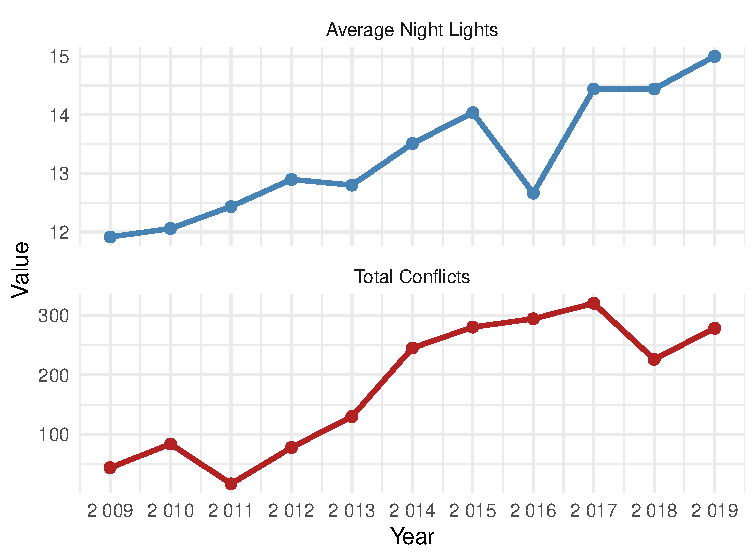
\includegraphics[width=0.8\textwidth]{aa.pdf}
	\caption{Conflict and nightlight}
	\label{nightl}
\end{figure}

\autoref{nightl} shows the patterns are consistent with dual influences. In 2013 and especially 2016, declines in nightlights coincide with marked increases in conflict, suggesting real economic disruption alongside potential measurement noise. \\
\begin{figure}[!htbp]
	\centering
	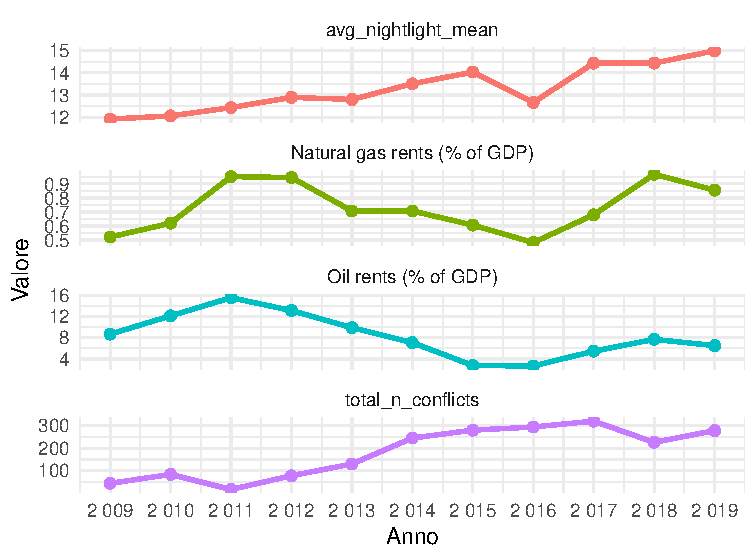
\includegraphics[width=0.8\textwidth]{sec.pdf}
	\caption{Confroning conflict, nightlight and different type of rent}
	\label{con}
\end{figure}

\autoref{con} shows a similar pattern and, in particolar, that the 2016 episode also aligns with a sharp fall in traded-goods rents
Those observations linked with the sensor moviment could explain the drop 
Of course, part of the discontinuity in nightlights reflects known sensor and constellation changes \textcite{li2020harmonization}. Yet the comovement we observe, nightlights falling in 2013 and especially 2016 while conflict rises and traded goods rents contract, suggests a substantive pattern beyond pure measurement noise. This alignment points to plausible real-economy disruption coinciding with the technical break. While we do not claim causality here, the repeated timing and direction of these series indicate a relationship that merits deeper investigation rather than being dismissed as a data artifact alone.
\chapter{Heterogeneity}
\label{app:descriptives}
This appendix provides additional information about the measurement used as heterogeneity employed used in the empirical strategy. \\
In our analyses we accounted for different spatial heterogeneity, in particular for geographic, sectorial, social and environmental one.\\

Starting from geographical dimension, we studied both the differences between East and Ovest and the ones between Nord and South. We costructed the dummies using respectively the longitude and latitude median. Nord and South, as shown in table \ref{tab:ns_summary}, display strong differences in nightlight concentrations, a proxy for economic activity: the South is brighter on average and more dispersed, while the North is dimmer and more stable. This suggests that in southern regions, the wealthiest areas are wealthier than those in the north. \\

\begin{table}[htbp]\centering
	\caption{Summary statistics by North/South macro-region}
	\label{tab:ns_summary}
	\resizebox{1\textwidth}{!}{
	\begin{tabular}{lc|c|c|c|c|c|c}
		\toprule
		Macro-region &$n$ & Mean NTL & SD NTL & Mean trade & SD trade & Mean conflicts & SD conflicts \\
		\midrule
		North & 748  & 1.35 & 0.885 & 9.07    & 50.0     & 0.707 & 1.89 \\
		South & 1232 & 2.59 & 0.932 & 131551.0 & 2782390.0 & 1.19  & 3.55 \\
		\bottomrule
	\end{tabular}
	}
	\vspace{3pt}
	\begin{minipage}{1\textwidth}
	\footnotesize Notes: NTL = log night-time lights. Trade = $indice2\_main$. Conflicts = number of consumption-related events.
	\end{minipage}
\end{table}


However, the corresponding regressions are not statistically significant, so we do not rely on the North/South split in the main analysis. \\
\clearpage
\begin{figure}[!htbp]
	\centering
	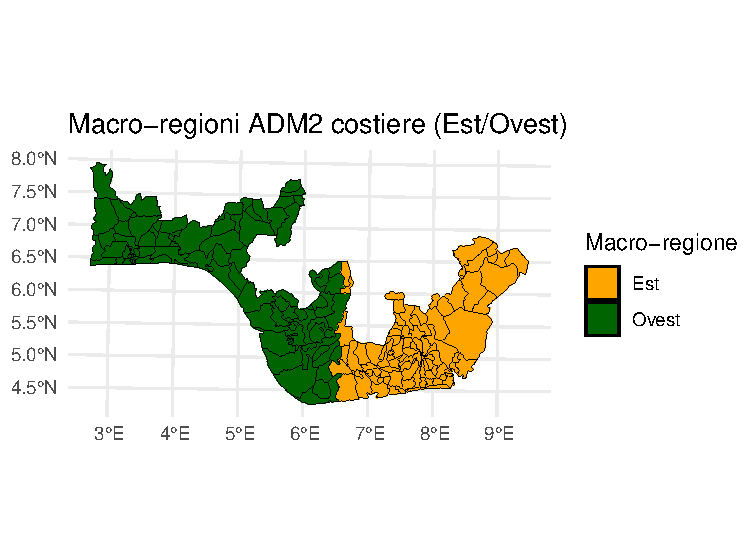
\includegraphics[width=0.7\textwidth]{est_ovest.pdf}
	\caption{est and ovest}
	\label{est}
\end{figure}

We therefore focus on the East West division. Figure \autoref{est} shows the spatial partition and, following the intuition of the Panel B of Table \ref{tab:ns_summary}, we analysed the logarithmic distribution of nightlights by macro region \autoref{est2}.\\

\begin{figure}[!htbp]
	\centering
	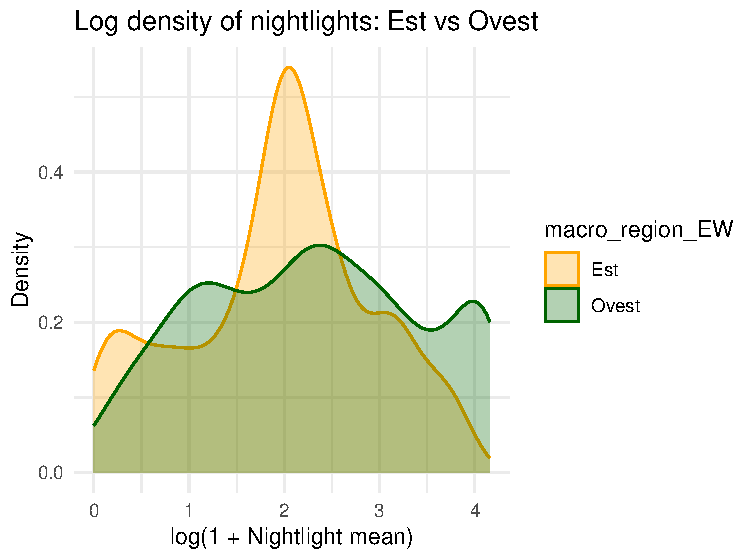
\includegraphics[width=0.7\textwidth]{log est_ovest.pdf}
	\caption{log density of nightlights}
	\label{est2}
\end{figure}
The pattern confirms our intuition: the East, in orange,  concentrates around ~2 with more mass at lower values, while the West, in green, features a heavier right tail up to ~4. This suggest that the western ADM2 units are, on average, brighter and more dispersed.\\

A noteworthy observation is the almost perfect symmetry between the geographic (East/West) and the sectoral dimensions (Import/Export and Vegetables-first/Chemicals-first): they cover largely the same ADM2 units, which strengthens the interpretation of our heterogeneity results.
This symmetries are shown in Figure \ref{est}, \ref{flow} and \ref{sector}


\begin{figure}[!htbp]
	\centering
	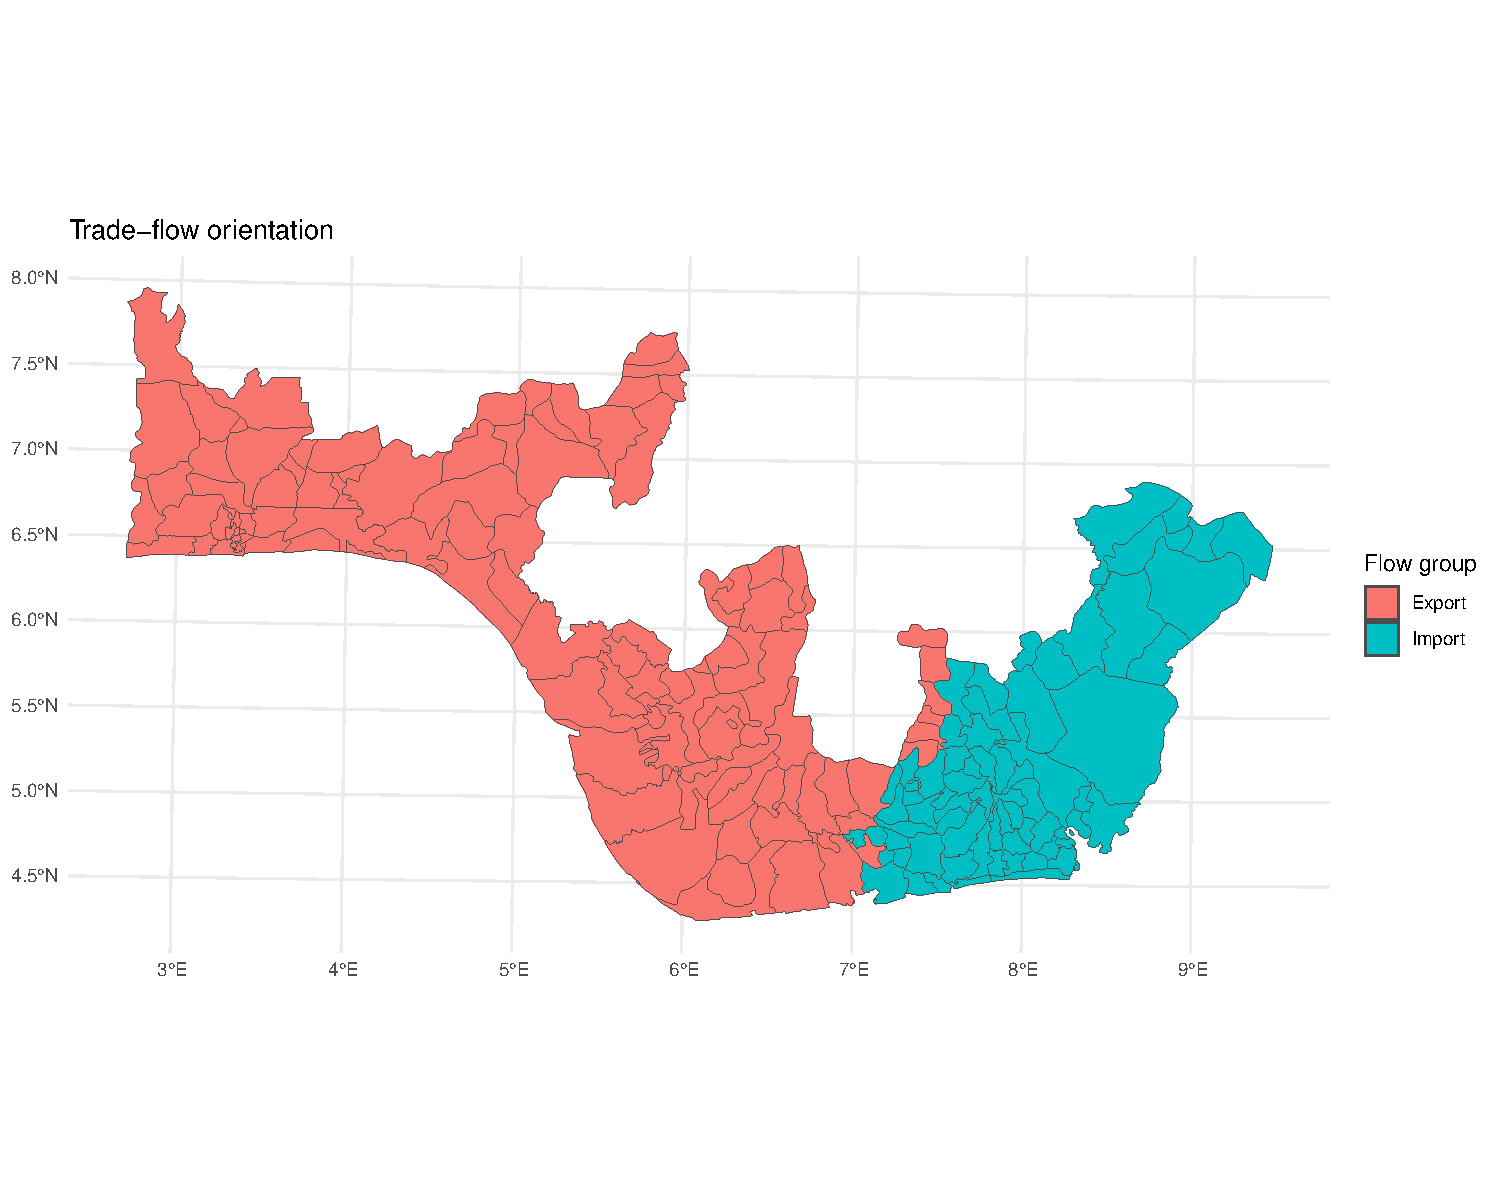
\includegraphics[width=0.7\textwidth]{flow.pdf}
	\caption{Import and export}
	\label{flow}
\end{figure}

\begin{figure}[!htbp]
	\centering
	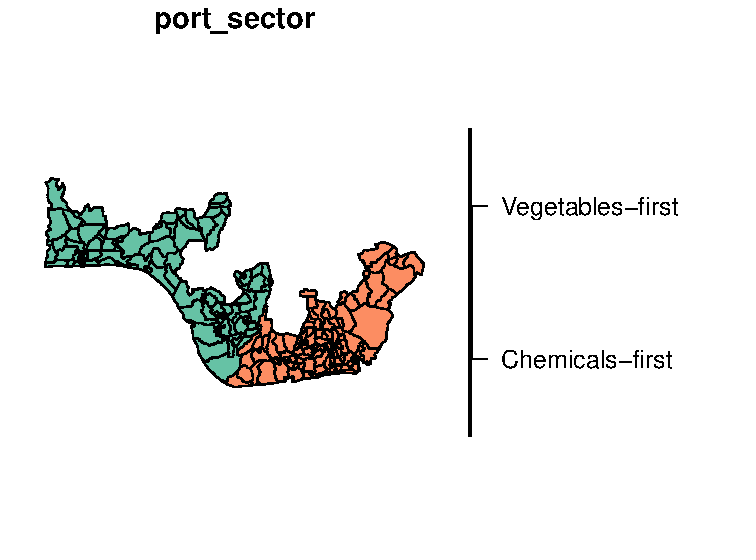
\includegraphics[width=0.7\textwidth]{sector.pdf}
	\caption{Vegetable and chemicals}
	\label{sector}
\end{figure}

\chapter{Replication Code}
% Short intro text (optional)
This appendix provides the R code used to construct the analysis
\lstinputlisting[
language=R,
caption={Full pipeline},
label={lst:pipeline-r}
]{code/main.R}


\newpage
\phantomsection
\addcontentsline{toc}{section}{Figure}

\begin{acknowledgments}
\chapter{Ringraziamenti}
Questa tesi è il frutto di ricerche e di lavoro svolto a conclusione della laurea magistrale.\\
Desidero, per primo, ringraziare il mio relatore, il Professor Valerio Leone Sciabolazza che mi ha fatto scoprire la mia passione per la ricerca e per l’economia dello sviluppo. Fin dal primo anno mi ha accompagnata con disponibilità e consigli preziosi, di cui farò tesoro.\\

Negli ultimi tempi molti paragonano la vita a un libro o a una serie TV (nel mio caso sarei al capitolo, o alla stagione, 24), ma non è un’immagine che sento davvero mia. Io penso alle persone che mi accompagneranno sempre, nel bene e nel male, e a quanto ho imparato da ciascuna e non riesco a vederli come personaggi secondari. Più che a un libro già scritto, preferisco paragonare la mia vita a un quaderno su cui continuo a scrivere: un quaderno un po’ particolare, che cambia stile a ogni pagina. Siamo noi, in fondo, a dare forma alle nostre avventure. \\
Sicuramente la mia famiglia è una di quelle cose su cui ho scritto e scriverò di più. Grazie a mamma e papà, che mi supportano nonostante non capiscano sempre le mie decisioni e che sono stati un riparo quando ne avevo bisogno. Fin da piccola mi hanno dato tutti gli strumenti per ritagliarmi un posto del mondo. \\
Grazie ai miei fratelli Francesco e Claudia. Non avremo il rapporto che spesso si vede nelle serie tv, ma negli anni ci stiamo avvicinando sempre di più. Grazie per aver "combattuto" molte battaglie al posto mio, ma anche grazie per avermi lasciato la possibilità di vincerne altre. Grazie Clo, per avermi insegnato che non si deve sapere tutto sempre dell'altra persona, ma che anche il silenzio vale molto e sopratutto per avermi insegnato che se si ha un obiettivo lo si può portare avanti costruendosi la propria strada. Grazie Checco per essere stato sempre sincero. Mi hai insegnato che se un'idea è giusta si deve combattere per cercare di realizzarla. Grazie per tutto l'aiuto con il codice, LaTex e per essermi stato vicino nei momenti di crisi (e, durante la tesi, non sono stati pochi). Insomma, grazie per l’esempio che mi avete dato, ciascuno a modo suo, nonostante le nostre differenze. Vi voglio bene. \\

Grazie a Fami Ohana, o famiglia padovana per meglio intenderci, che anche da lontano sono sempre i primi a festeggiare qualsiasi traguardo. Grazie zia Mock e zio Giovanni che mi fate ridere come non mai quando stiamo insieme, grazie zio Alberto che riesce sempre a farmi tornare bambina e grazie Zio Andrea e zia Caterina per essere presenti. Grazie Nonna Pia, mi hai insegnato moltissimo in questi anni, mi hai insegnato tantissimo in questi anni; grazie per essere sempre disponibile quando ti chiamo e per i consigli che mi dai. Sarai una nonna un po’ “atipica”, ma sei piena di vita e mi hai mostrato che, se si tiene la mente allenata, si può fare qualsiasi cosa si voglia. Un ringraziamento speciale a Nonno Nildo, che è sempre nei miei pensieri e che mi manca moltissimo. \\

Oltre la famiglia padovana, voglio ringraziare i miei vicini di casa, la famiglia tiburtina. Sono dei vicini un po' particolari, ma su cui si può sempre contare per qualsiasi cosa. Grazie Luigi, perchè sai sempre come strapparmi un sorriso, a casa sarà sempre presente un caffè con il dolcificante. Grazie zia Giò, i tutto: per essere sempre disponibile, anche nelle emergenze all’ultimo; per cercare di capirmi e sostenermi, ma anche per dirmi quando non sei d’accordo con me. Grazie, perché so che, anche se sono lontana e non chiamo spesso, sai che ti voglio bene. Ho tantissimi ricordi del tempo passato insieme: sono custoditi nel mio cuore, anche quando può sembrare che me ne dimentichi. Un grazie speciale anche a Nonna Maria, l'unica che è riuscita a farmi mangiare le verdure (fritte e pastellate) e che ricorderò sempre con la sua collana di perle e il sorriso. \\

Come tutti sappiamo, la famiglia non è fatta solo di legami “di sangue”: la famiglia si sceglie. Io la mia l’ho scelta molto tempo fa, o meglio, non l’ho scelta davvero, ed è questa la cosa più bella.\\
C'è una persona che è stata una costante nella mia vita, che mi ha fatto conoscere libri, serie, musica ma anche vivere avventure insieme. La mia persona. Carola. Mi sei stata vicina in tutti i momenti difficili, e in quelli bellissimi. Grazie Caro per avermi insegnato tanto e, onestamente, non saprei nemmeno da dove iniziare. Sei quella persona che, anche se non ci sentiamo per un mese, quando ci rivediamo è come se non fosse passato un giorno. Mi hai sempre incoraggiata a sfidare le mie capacità e a credere in me stessa, senza farmi fermare dalla paura di fallire. Con te passerei un'intera giornata a non fare nulla, solo a stare insieme: la tua compagnia mi fa stare bene, mi ricarica. La cosa che amo di più è venire a cena da te e cantare/gossippare mentre cucini. Grazie perchè senza il tuo supporto non avrei fatto metà delle cose che ho fatto, e di certo non sarei arrivata fin qui. Insieme abbiamo vissuto tantissime imprese e non vedo l'ora di viverne altre. Con te posso essere me stessa, e questo basta a rendere semplice perfino il silenzio. Come ti avevo detto tempo fa "voglio passare i vent'anni con te". Stiamo \textit{quasi} a metà percorso e continuo a pensare che non potessi scegliere meglio.\\

Ci sono delle persone con cui poi sono cresciuta insieme, anche se abbiamo preso strade molto diverse. Tizi e Mils, grazie per essere sempre voi stesse. Grazie Tizi per la tua spontaneità e ironia e Mils per la tua determinazione e per essere sempre solare. \\

Oltre alle amicizie storiche ce ne sono alcune che ho fatto nel percorso universitario e che hanno reso quest'esperienza unica. La prima fra tutti Sab. Ti ho conosciuta nel post-Covid, dopo un esame, per caso: la casualità migliore che potesse capitare. Sei stata un punto fermo, una persona con cui potevo essere sempre diretta. Mi hai insegnato a non arrendermi, che la propria strada si costruisce passo dopo passo e che nessuno, se non noi stesse, può giudicare le nostre scelte. Sono fiera della persona che sei diventata e io so che nessuno ti può fermare. Grazie per essermi stata vicina e aver saputo sempre cosa dire. \\
Insieme a Sab quell'anno ho conosciuto Alessio e Samuele, due colleghi universitari che non potrebbero essere più diversi tra loro. Ale, grazie perché sei sempre diretto e perché so che, se uno dei due ha bisogno, l’altro si farebbe in quattro. Le Pasquette più divertenti della mia vita portano il tuo nome. Sarò sempre qui per quando avrai bisogno. Samu, sei un paradosso per me, sei la persona più organizzata che conosco ma contemporaneamente quella più disorganizzata: ogni tanto scopro cose diverse che fai e non smetti mai di sorprendermi. Grazie per essere sempre stato un buon amico (e anche una buona spalla).\\ Sono davvero felice di aver passato questi 5 anni con voi ragazzi. \\

Grazie a Marco e Giovanni, due amici conosciuti l'ultimo anno di triennale che mi hanno cambiato completamente la visione dell'università. Gio, grazie per gli aperitivi e i caffè in cui mi fai morire dal ridere. Marco, te che ti metti in discussione ogni tre per due. Sei una persona fantastica, genuina, di quelle rare. Te che hai letteralmente deciso di adottarmi quando mi ha visto persa per i corridoi dell'università. Grazie, senza di te avrei perso tantissimo. \\

Grazie a EPOS sub ITA, senza che nomino tutti. Le lezioni grazie a voi sono state molto più leggere. Ci sono dei nomi speciali però che vorrei ringraziare: grazie Lucri, che nella tua ansia mi tranquillizzavi. Grazie per avermi fatta sentire capita fin da subito pisi. Grazie Bi, la tua gentilezza e il tuo ottimismo sono stati i motori di questi miei due anni, insieme ai nostri audio cortissimissimi. Da quando ti conosco non smetto di dire "ma è un cucciolo" e lo trovo bellissimo. Grazie Ale, sei stato un compagno di scleri, di "te hai iniziato?" "si sono a capitolo 5, te?" "no..." "a vabbè ma ce la fai". Sei una persona sincera, sorridente, non smettere di esserlo. Grazie Nora, per incoraggiarmi sempre e per capirmi al primo sguardo. Grazie di tutto ragazzi.  \\
Grazie a Francesco, che mi ha supportato e creduto in me sempre, soprattutto quando volevo mollare. Ha saputo incoraggiarmi, aiutarmi e ha sopportato molte, forse quasi troppe, mie sclerate relative sia all'università che non. Sei stato una sorpresa e mi hai insegnato che tutto si risolve, sempre: non tutto è grave come lo percepiamo e non tutto va preso sul serio. Grazie per ripetermi sempre: "una cosa alla volta, un passo dopo l'altro" quando mi sento troppo piena di cose da fare. Mi hai fatto riscoprire l'amore per l'economia, quella però più quotidiana, non solo quelle teorie che studiamo sui libri. Grazie perché so che posso contare su di te sempre, sopratutto quando non credo in me. Sei stato un punto di riferimento senza il quale avrei sicuro perso la rotta, e già io non ho un buon senso dell'orientamento. Il tuo sostegno in questi anni, ma sopratutto durante la stesura della tesi, è stato fondamentale. Grazie. E ricorda "tantissimo".\\

L'università, però, non è solo studio. E chi mi conosce lo sa, non perdo mai l'opportunità di riempirmi di cose da fare, sennò poi come mi lamento? \\
Proprio in università ho incontrato un mondo a cui non avrei mai pensato di appartenere e che, da spettatrice, avevo sempre ammirato. Casualmente, infatti, un giorno scopro che c'era una certa associazione che organizzava il TEDx Universitario. a scelta più pazza che potessi fare: io a organizzare eventi, a parlare con le aziende per ottenere fondi e riconoscimenti, a cercare tirocini tra il pubblico… io, che mi agito a scrivere un’email al professore.\\
Invece sono entrata, ed è stato amore a prima vista, ma sopratutto ho conosciuto delle persone stupende. \\
Per prima, Sabrina, che mi ha accolto a casa. Sei stata la presenza più importante del mio percorso associativo: una spalla quando tremavo, una consigliera quando serviva lucidità. Ci siamo conosciute online e, pagina dopo pagina, ti sei fatta spazio nel mio cuore. Ogni volta che ci vediamo il tempo corre troppo in fretta: sono grata di averti incontrata e di aver avuto la possibilità di conoscerti. Io sarò qui, a tifare per te, sempre. E poi… hai visto? Ho preparato una presentazione! \\
Oltre Sabrina, un grazie va a tutto il team ERS: Cecilia, Nicoletta e Matteo (e anche a chi ci siamo persi per la via). Ragazzi, non ho più parole per dire quanto sono orgogliosa di noi, del nostro percorso e del rapporto che abbiamo costruito. A prescindere so che riuscirete a fare ancora meglio. Mi mancheranno le nostre call, le strategie pensate insieme e anche i dibattiti su come rispondere alle richieste insolite degli sponsor.\\
Un grande grazie va anche al consiglio direttivo che mi ha sostenuta e insegnato tantissimo, accompagnandomi nel mio percorso. In particolare, grazie Silvia per aver sempre creduto in me e avermi consigliato, anche tardi la notte. Grazie per il sostegno: sei stata una bussola nei momenti confusi e una spinta quando avevo paura di fermarmi. Sei una persona speciale, che sa sempre cosa dire e ha una visione della vita stupenda, anche se diversa dalla mia. Con te mi sono sentita capita e al sicuro. Sono contenta di poterti considerare amica \\
Il TEDxSapienzaU non sarebbe lo stesso senza di voi. \\

A chi mi ha accompagnata fin qui: questa pagina porta anche la vostra firma.\\
Questa non è la fine del mio racconto, è una virgola. Il viaggio continua. Una cosa alla volta, un passo dopo l’altro: il mio quaderno resta aperto. Grazie
\end{acknowledgments}

\end{document}